\documentclass[10pt,a4paper,twoside]{article} 
\usepackage[latin1]{inputenc}
\usepackage[english]{babel}
\usepackage{amsmath}
\usepackage{amsfonts}
\usepackage{amssymb}
\usepackage{makeidx}
\usepackage{graphicx}
\usepackage{hyperref}
\usepackage[left=2cm,right=2cm,top=2cm,bottom=2cm]{geometry}
\usepackage{float}
\usepackage{multirow}
\usepackage{verbatim} %for å kommentere ut ting
\usepackage[nottoc,numbib]{tocbibind}
\usepackage[parfill]{parskip} %for avsnitt
\usepackage{listings}
    \lstset{
            language=Matlab,                                % choose the language of the code
    %       basicstyle=10pt,                                % the size of the fonts that are used for the code
            numbers=left,                                   % where to put the line-numbers
            numberstyle=\footnotesize,                      % the size of the fonts that are used for the line-numbers
            stepnumber=1,                                           % the step between two line-numbers. If it's 1 each line will be numbered
            numbersep=5pt,                                  % how far the line-numbers are from the code
    %       backgroundcolor=\color{white},          % choose the background color. You must add \usepackage{color}
            showspaces=false,                               % show spaces adding particular underscores
            showstringspaces=false,                         % underline spaces within strings
            showtabs=false,                                         % show tabs within strings adding particular underscores
    %       frame=single,                                           % adds a frame around the code
    %       tabsize=2,                                              % sets default tabsize to 2 spaces
    %       captionpos=b,                                           % sets the caption-position to bottom
            breaklines=true,                                        % sets automatic line breaking
            breakatwhitespace=false,                        % sets if automatic breaks should only happen at whitespace
            escapeinside={\%*}{*)}                          % if you want to add a comment within your code
    }

\raggedbottom

\usepackage{makeidx}
\makeindex
%symbolliste slutt

\author{Anders Dall'Osso Teigset}
\title{MEDIUM VOLTAGE LOAD BREAK SWITCH WITH AIR AS INTERRUPTING MEDIUM}
\date{December, 2013}


\begin{document}
    \begin{titlepage}
    \begin{center}
    \ \\
    \ \\
    \ \\
    \ \\
    \ \\
    \ \\
    Anders Dall'Osso Teigset \\
    \ \\
    \ \\
    \ \\
    \ \\{\large \bfseries
    MEDIUM VOLTAGE LOAD BREAK SWITCH WITH AIR AS INTERRUPTING MEDIUM\\
    }
    \ \\
    \ \\
    \ \\
    \ \\
    \ \\
    {\large
    Specialisation project\\
    }
    \ \\
    {December, 2013 \\}
    \ \\
    \ \\
    \ \\
    \ \\
    \ \\
    \ \\
    \ \\
    \ \\
    \ \\
    \ \\
    \ \\
    \ \\
    \ \\
    \ \\
    \ \\
    \ \\
    \ \\
    \ \\
    \ \\
    \ \\
    \ \\
    \ \\
    \ \\
    \ \\
    \ \\
    \ \\
    \ \\
    \ \\
    \ \\
   	{\large
   Norwegian University of Science and Technology\\
   Department of Electric Power Engineering\\
    }
   	\ \\
    \ \\
    \ \\
    \ \\
    \end{center}
    \end{titlepage}

%\maketitle
%SummaryNyttige pdf-filer/SF6conduct.pdf
\thispagestyle{empty}
\cleardoublepage
\section*{Acknowledgements}
\setcounter{page}{1}
\pagenumbering{roman}

\cleardoublepage
\section*{Summary}

\cleardoublepage
\setcounter{page}{1}
\pagenumbering{arabic}
\tableofcontents
\cleardoublepage

\section{Introduction}

\cleardoublepage

\section{Theory}
\subsection{Typical switchgear design and interruption sequence} \label{sec:genDes}
Most of the information in section \ref{sec:genDes} is collected from \textit{"Current Interruption in Power Grids"} by Magne Runde \cite{bib:HVEbreak} \newline

\subsubsection{Switchgear design and operation} \label{sec:InterruptCurrent}
Switchgear can be divided into four main categories:
\begin{itemize}
\item Disconnector Switch
\item Load Break Switch
\item Circuit Breaker
\item Earthing Switch
\end{itemize}

This report will focus on the load break switch (LBS) design. An LBS is designed to be able to interrupt currents with a magnitude that is equal or less than the rated maximum continuous current in a transmission system. An LBS should fulfil the following demands to meet the requirements of the application area:

\begin{itemize}
\item When closed:
	\begin{itemize}
		\item It must act as an good conductor.
		\item Be capable of interrupting any load that may arise, without generating too high over-voltages. 
	\end{itemize}
\item When open:
	\begin{itemize}
		\item It should act as a close to perfect insulator.
		\item Be able to close without welding the contacts together, even under short-circuit conditions.
	\end{itemize}
\end{itemize}

A typical operation sequence for a switch is as follows. First a control signal enters the switch and activates the driving mechanisms, in most cases this is a compressed spring or a hydraulic-system. The contacts starts to open and a gap forms between them. At the same time, an electrical arc ignites between the contacts, burning in the gap. The gap is filled with some kind of interrupting medium which is usually a gas. For a alternating current with a frequency of 50 Hz the current will cross zero 100 times per second, and this crossing is called the current zero (CZ). Direct current interruptions will not be explained in this report.

At the CZ the arc will extinguish, for at least a moment, because the current is zero, and a voltage will build up between the contacts. This voltage is called the recovery voltage and is defined in equation \eqref{eq:U_rec}, where $u_{supply}$ is the voltage on the supply side and $u_{load}$ is the voltage on the load side of the open switch. Depending on the recovery voltage two possible scenarios can occur: a re-ignition or a quenching of the arc. This is dependent on the rate of raise and the amplitude of the recovery voltage. There are two different kinds of re-ignition: thermal and dielectric. Thermal re-ignition takes place right after CZ, up to a few microseconds, and is mainly dependent on the steepness of the recovery voltage. As the recovery voltage rises and if a thermal re-ignition is avoided, a dielectric re-ignition may occur. This kind of re-ignition is largely dependent on the amplitude of the recovery voltage and will occur after a millisecond or more. This paper will mainly focus on thermal re-ignition. The likelihood of a re-ignition  will not be de-terminated by the arcing voltage it self, but how the interrupting medium which is used reacts on the arcing voltage. Important interruption properties of air is featured in section ???. Other design parameters like contact material, geometry, contact moment speed, and cooling mechanisms are also important to the interruption properties.

\begin{equation} \label{eq:U_rec}
u_\mathrm{{recovery}}=u_\mathrm{{supply}}-u_\mathrm{{load}}
\end{equation}  

Plasma is generated when gas and metal vapour is heated to very high temperatures. At a certain point, the molecules in the gas decomposes to ions and free electrons. This mixture is called plasma, and makes up most of the components an electrical arc burns in, except for arcs that burns in vacuum. Vacuum arcs will not be featured in this report.

In most switchgear designs it is common to have two contact sets, one called the main contact and the other is called the arcing contact. The main contact is the first contact to open and the last one to close. This is to ensure that an arc does not start to burn between the main contact. The arcing contact is the last contact to open, and the first one to close, and will ensure that the arc burns between the arcing contact and not between the main contact.

Since the main contact open first, and closes last its main purpose in the switchgear is to act as an good conductor. Copper or aluminium are good materials and are commonly used to ensure that this aspect of the switch is met. Sometimes, the contact surface is plated with tin, gold, silver, or platinum to ensure an even lower contact resistance between the contacts. The main problem with electrical losses in the switch is heat generation, which may speed up metal creep and other ageing-related processes in the switch. Contacts made of aluminium are especially vulnerable to creeping.

The arcing contacts are designed to withstand the harsh conditions that occur when an arc burns between the contacts. The contact material has to meet strict requirements and has to tolerate high temperatures and arc erosion, and avoid welding and other stresses that may apply when closing or opening an energized contact. Aluminium and copper are not fit for these tasks since they will melt or erode from the stresses of an arc. It is common to use composites that consists of metals with good electrical conduction and heat-resistant oxides. For high current and voltage switches, it is possible to use a composite of silver or copper together with tungsten or tungsten carbide. These materials are highly heat-resistant, but they also have a high electrical resistance. The higher electrical resistance in the arcing contact compared to the main contact is however, not a problem, since the current only flows through the arcing contact for a short period of time.

\subsubsection{The puffer principle}

   
\subsubsection{Heat transportation in an arc} 


\subsubsection{The difference between air and SF$_6$ as interrupting medium} 



\subsubsection*{Electrical conductivity}


\subsubsection*{Thermal conductivity}


\subsubsection*{Dielectric properties} 


\subsubsection*{Chemical properties}


\subsection{Environmental impacts of SF$_6$ from electrical power industries} 


\cleardoublepage

\section{Method}

\subsection{Test circuit} \label{sec:testCir}

Figure \ref{fig:testSwitchRiggEq} illustrates the physical appearance of the test switch. The numbered parts are: 1. Compressed air reservoir (connected to the high voltage supply circuit), 2. Tulip contact, 3. Nozzle, 4. Pin contact, 5. Connection to load circuit, 6. Spring drive mechanism, 7. Electromagnet release mechanism, and 8. Position transducer.

\begin{figure} [H]
\centering
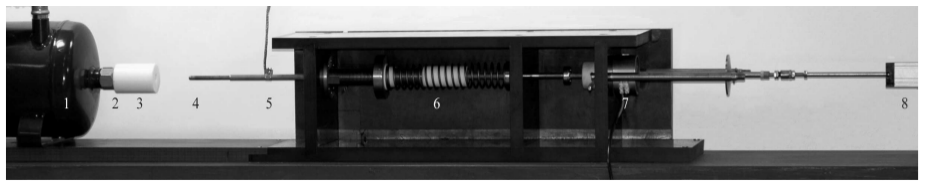
\includegraphics[scale=0.5]{Bilder/Method/switchTest.png}
\caption{The physical appearance of the test switch \cite{bib:AFIMVLBA}.} \label{fig:testSwitchRiggEq}
\end{figure}

Figure \ref{fig:testCurcuit} displays the laboratory test circuit used for the interruption tests. The circuit is designed to supply a 50 Hz / 13.8 kV current. It is possible to shape the TRV by tuning the parameters: L$_1$, L$_s$, R$_1$, R$_d$, and C. The systems' short circuit parameters are R$_{sc}$ and L$_{sc}$. The TRV generated during interruption is set to simulate the standard for a 24 kV / 630 A class from the International Electrotechnical Commission (IEC), which corresponds to:

\begin{itemize}
\item The initial part of the TRV has a rate of rise in recovery voltage (RRRV) of 71 - 73 V / $\mu$s.
	\begin{itemize}
		\item The voltage difference is measured over the first 20 $\mu$s after CZ.
	\end{itemize}
\item The first voltage peak is between 7.0 and 7.4 kV, with a rise time of approximately 96 $\mu$s.
\end{itemize}

\begin{figure} [H]
\centering
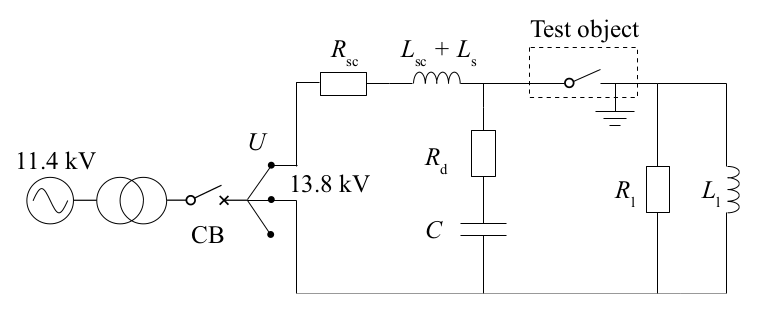
\includegraphics[scale=0.35]{Bilder/Method/circuit.png}
\caption{Circuit used for the interruption test \cite{bib:AFIMVLBA}.} \label{fig:testCurcuit}
\end{figure}

In table \ref{tab:testParameters}, the value of the different test circuit parameters and the corresponding current can be observed. The test is conducted at currents with an RMS value of 630 A and 880 A. In the entire experiment the TRV is kept constant up to and including the first voltage peak. In the case of a failed interruption a thermal re-ignition occurs within a few microseconds after CZ.

\begin{table}[H]
\center
\caption{Circuit Parameters and Resulting Current \cite{bib:AFIMVLBA}. }
\begin{tabular}{|c|c|c|c|c|c|}
\hline 
L$_s$ [mH] & L$_1$ [mH] & R$_1$ [$\Omega$] & C [nF] & R$_{d}$ [$\Omega$] & I [A] \\ 
\hline 
6.9 & 86.2 & 22.1 & 102 & 198 & 630 \\ 
\hline
2.9 & 60.2 & 15.1 & 156 & 170 & 880 \\
\hline   
\end{tabular} 
\label{tab:testParameters}
\end{table}

A resistive transducer is measuring the contact position while a Hall Effect current transducer is measuring the current through the test switch. The voltage between the contacts is measured with a parallel resistive / capacitive voltage divider. All measurements are transmitted through optical fibres to a 12 bit resolution transient recorder with a sampling frequency of 2.5 MHz. The pressure in the tank is only measured before each test with an accuracy of 0.01 bar.

\subsection{The switch and contact geometry}
This experiment is conducted using copper-tungsten arcing contacts, polytetraflourelthylene (PTFE) nozzles, and air as interrupting medium. It is an open system, with the surrounding air at atmospheric pressure \textit{p$_0$} and a six-litre tank with a pre-filled upstream overpressure \textit{p$_u$}, used during the interruption process to quench the arc. It is possible to adjust the upstream pressure, contact speed, and position at current zero (CZ) independently, as well as the contact and nozzle geometry. The current and transient recovery voltage (TRV) can be change by changing the parameters of the laboratory test circuit, as described in section \ref{sec:testCir}.


A simple drawing of the contact and nozzle is displayed in figure \ref{fig:contactAndNozzle}. The length of the nozzle is 20 mm, and the inner diameter is \textit{D}, axial symmetry is present along the x-axis. Two different contact geometries are going to be tested, denoted a and b. The dimensions of the different geometries are given in table \ref{tab:contGeoPara} and, how the different dimensions are defined is illustrated in figure \ref{fig:AreacontactAndNozzle}. The angle $\mathrm{\theta}$ is defined so that $A_\mathrm{{funnel}}=4 \cdot A_\mathrm{{nozzle}}$ for each geometry.

The contact position \textit{x} is defined as the axial distance between the tulip and the pin contact. At starting position, \textit{x}= -60 mm and the pin contact is acting as a plug for the tank. This is making it possible to pre-set an upstream pressure. The contact is held in place by an electromagnet and is set to motion when the magnet releases a compressed spring. The spring accelerates the pin contact up to a speed of approximately 5.5 m/s at \textit{x}=0. At this position, the spring is unloaded and the pin moves with a constant speed until the contact is fully open at \textit{x}=110 mm.

\begin{figure} [h]
\centering
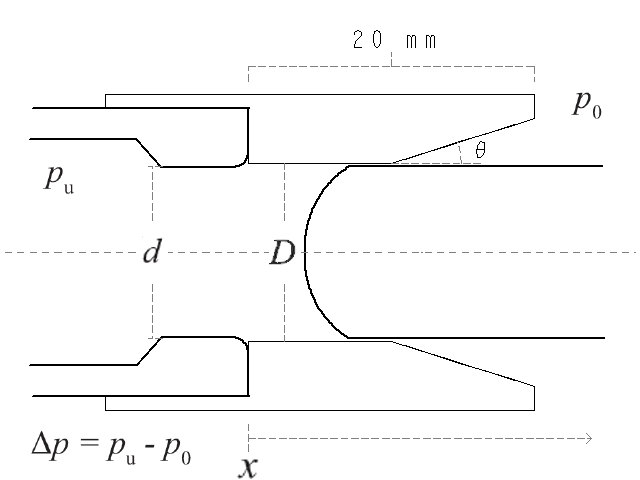
\includegraphics[scale=0.45]{Bilder/Method/ContactAndNozzleFunnelShape5.png}
\caption{The contact and nozzle. The diameter of the contact is \textit{d} and the inner diameter of the nozzle is \textit{D}.} \label{fig:contactAndNozzle}
\end{figure}

\begin{figure} [H] %denne må byttes ut.
\centering
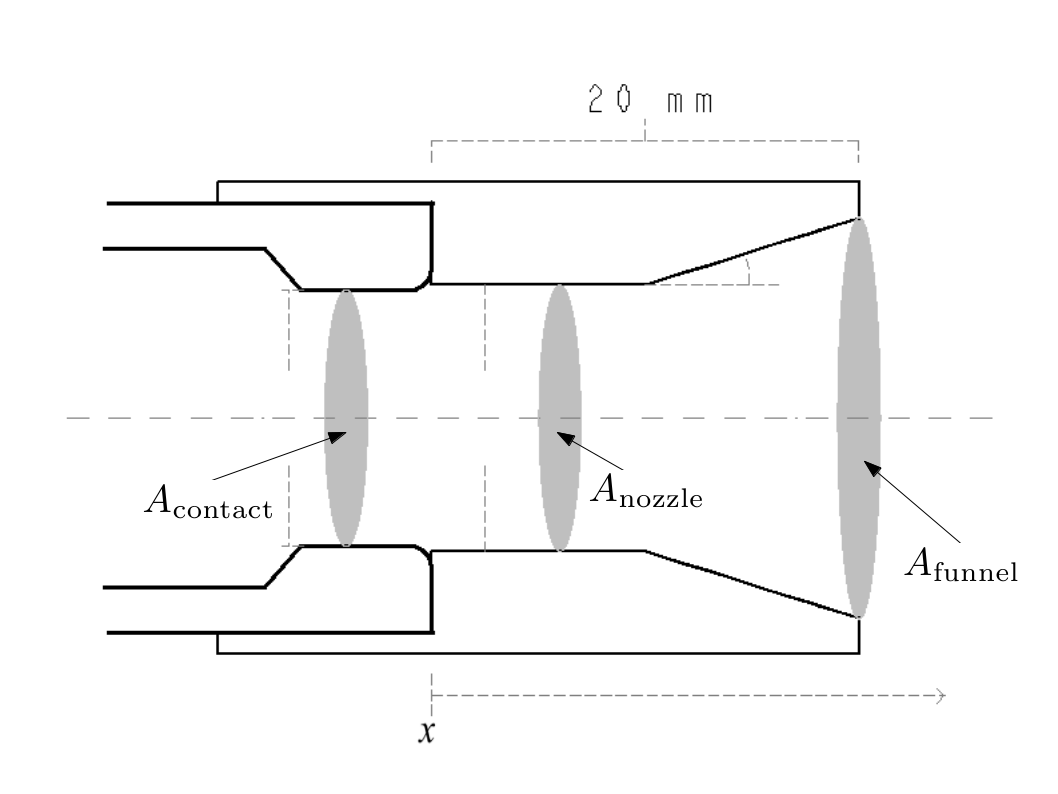
\includegraphics[scale=0.35]{Bilder/Method/AreaDef.png}
\caption{Overview over how the different areas are defined.} \label{fig:AreacontactAndNozzle}
\end{figure}

\newpage
\begin{itemize}
\item $A_\mathrm{{contact}}$ is the cross section of the contact pin, as well as the area of the tulip contact. The area is described by equation \eqref{eq:A_contact}.

\item $A_\mathrm{{nozzle}}$ is defined as the area of the cylindrical part of the nozzle, when x=[0,10] mm. The area is described by equation \eqref{eq:A_nozzle}.

\item $A_\mathrm{{funnel}}$ is defined as the area at the end of the nozzle, when x=20 mm, and the diameter of the funnel is at its biggest. This area is described by equation \eqref{eq:A_funnel}.

\item $A_\mathrm{{ring}}$ is in table \ref{tab:contGeoPara} defined as the area between the pin contact and the cylindrical part of the nozzle, when x=[0,10] mm and is described by equation \eqref{eq:A_ring_1}. For x=[10,20] mm $A_\mathrm{{ring}}$ is a function of the pins position, x, inside the nozzle, described by equation \eqref{eq:A_ring_2}.
\end{itemize}

\begin{equation} \label{eq:A_contact}
A_\mathrm{{contact}}=A_\mathrm{{tulip}}=\pi \frac{d^2}{4}
\end{equation}
\begin{equation} \label{eq:A_nozzle}
A_\mathrm{{nozzle}}=\pi \frac{D^2}{4}
\end{equation}

\begin{equation} \label{eq:A_funnel}
A_\mathrm{{funnel}}=4 \cdot A_\mathrm{{nozzle}}=4\pi \frac{D^2}{4}
\end{equation}

\begin{equation} \label{eq:A_ring_1}
A_\mathrm{{ring}}=A_\mathrm{{nozzle}}-A_\mathrm{{contact}}=\pi\left( \frac{D^2}{4}-\frac{D^2}{4}\right)
\end{equation}
\begin{equation} \label{eq:A_ring_2}
A_\mathrm{{ring}}(x)=\pi\left( \left(\frac{10-x}{\sin (\theta)}+\frac{D}{2}\right)^2-\frac{D^2}{4}\right)
\end{equation}

\begin{table}[H]
\center
\caption{Contact geometry parameters.}
 \begin{tabular}{|c|c|c|c|c|c|c|c|c|}
\hline 
Geometry & D [mm] & d [mm] & $\frac{D}{d}$ & $\mathrm{\theta}$ & $A_\mathrm{{contact}}$ [mm$^2$] & $A_\mathrm{{ring}}$ [mm$^2$] & $A_\mathrm{{nozzle}}$ [mm$^2$] & $A_\mathrm{{funnel}}$ [mm$^2$]\\ 
\hline 
a & 6.25 & 6.0 & 1.04 & 17.4 & 28.3 & 2.4 & 30.7 & 122.8\\ 
\hline 
b & 7.40 & 7.0 & 1.06 & 20.3 & 38.5 & 4.5 & 43.0 & 172.0\\ 
\hline 
\end{tabular} 
\label{tab:contGeoPara}
\end{table}

\newpage
\subsection{Procedure}
Interruption tests with CZ occurring both inside and outside the nozzle are carried out, in total four tests are conducted in this interruption experiment. One test consists of one contact geometry at a current magnitude of either 630 A or 880 A with a minimum of five interruptions inside the funnel part of the nozzle and five interruptions outside the nozzle at each pressure level, and at least three different pressure levels are included in each test. Both the first and second CZ is included in this study to provide as much data as possible.

"Inside funnel" is defined as contact position x = [10, 20] mm and "outside nozzle" as x = [20, 60] mm at first CZ. Results from zero crossings that occurs in the cylindrical part of the nozzle, x $<$ 10 mm, between the tulip contact and the start of the funnel-shaped nozzle is discarded. The first CZ occurred within x $<$ 60 mm and the second CZ occurred for x $>$ 60 mm, as the contact speed during all tests was 5.5 mm/ms $\pm$ 0.5 mm/ms. When testing the interrupting capabilities inside the funnel the first CZ is aimed to occur at x=15 mm and when testing outside the nozzle the first CZ is aimed at x=30 mm. Due to variation in the travelling speed of the contacts some difference in the position of the pin at the moment of CZ will be present between each interruption attempt.

When testing the interrupting capabilities, the test procedure for each of the four cases was as follows: 

\begin{itemize}
\item[1.] A pressure level that seems to be in the area of interest is found by performing some initial test interruptions at different pressure levels. This level is kept constant for at least five interruption tests.
\item[2.] If a pressure level results in less than 100\% successful interruptions, at least five new tests with a higher upstream pressure (next level) are conducted. This is repeated until at least one pressure level with five successful interruptions is found.
\item[3.] Then, the pressure is stepped down until 60\% or more of the interruption attempts fail or the lowest possible pressure level is tested.
\end{itemize}

When testing for variations in the arcing voltage between a successful and unsuccessful interruption, a pressure level where the interruption success rate is 50 \% is used. Then five successful interruptions and five unsuccessful interruptions are obtained while the arcing voltage is measured and stored for further use. All the interruptions should occur outside the nozzle. The switching process is filmed by a high-speed camera so that the path of the arc can be monitored during the interruption.

The pin is cleaned, polished, and greased between each test to ensure a smooth surface. The contacts and nozzle are replaced regularly to avoid contact wear and nozzle deformation. This is to ensure that the geometry is constant through the whole experiment.
\cleardoublepage

\section{Results}
\subsection{Interruption tests} 


\newpage
\subsection{Arcing voltage}


\newpage
\subsection{Durability of the arcing contacts} \label{sec:durability}



\cleardoublepage

\section{Discussion}
\subsection{The probability of interruption} 


\subsection{Arcing voltage considerations}
 

\subsection{Durability of the arcing contacts} \label{fig:durability}


\newpage
\subsection{Suggestion for further work}
\subsubsection{A nozzle that minimises arc impact on air flow}


\subsubsection{Cone-shaped nozzle}


\cleardoublepage

\section{Conclusion}


\cleardoublepage
\begin{thebibliography}{10}
\bibitem{bib:SF6PI} L.G. Christophorou, J. K. Olthoff, and R.J. Van Brunt, "Sulfur hexafluoride and the electric power industry", \textit{IEEE Electrical Insulation Magazine, vol. 13, No. 5, pp. 20-24}, Oct. 1997.

\bibitem{bib:comSub} amesimpex.com, \url{http://www.amesimpex.com/images/unitised_sub_002.jpg}, 26.9.2013

\bibitem{bib:HVEbreak} M. Runde, "Current interruption in power grids", Trondheim: Norwegian University of Science and Technology, 2013

\bibitem{bib:CBAC} W. Rieder, "Circuit breakers, physical and engineering problems, III-Arc-medium considerations", \textit{IEEE spectrum, pp. 80-84}, Sept. 1970.

\bibitem{bib:IPSF6AQM} W. Hertz, H. Motschmann and H. Wittel, "Investigations of the properties of SF$_6$ as an arc quenching medium", \textit{Proceedings of The IEEE, vol. 59, NO. 4, pp. 485-492}, April 1971.

\bibitem{bib:TDCIGBB} W. Hermann, "Theoretical description of the current interruption in HV gas blast breakers", \textit{IEEE Transactions on Power Apparatus and System, vol. PAS-96, NO. 5, pp. 1546-1555}, Sept./ Oct. 1977.

\bibitem{bib:THFD} R. W. Johnson, "The handbook of fluid dynamics", Heidelberg: Springer-Verlag GmbH \& Co. KG, 1998.

\bibitem{bib:TET4160HVIM} E. Ildstad, "High voltage insulation materials", Trondheim: Norwegian University of Science and Technology, 2012, August 2012.

\bibitem{bib:KlimaKur2020} "KLIMAKUR2020", Oslo: Klima- og forurensningsdirektoratet, 2010

\bibitem{bib:consSF6} esrl.noaa.gov, \url{http://www.esrl.noaa.gov/gmd/webdata/iadv/ccgg/graphs/pdfs/ccgg.MLO.sf6.1.none.discrete.all.pdf}, 17.10.2013

\bibitem{bib:regSF6Miljo} regjeringen.no, \url{http://www.regjeringen.no/nb/dep/md/dok/regpubl/stmeld/2011-2012/meld-st-21-2011-2012/5/5.html?id=682932}, 21.10.2013

\bibitem{bib:StatSF6} K. L. Hansen, "Emissions from consumption of HFCs, PFCs and SF$_6$ in Norway", \textit{Statistics Norway/Department of Economic Statistics/Environmental Statistics}, 2007.

\bibitem{bib:AFIMVLBA} N. S. Aanensen, E. Jonsson, and M. Runde "Air flow investigation for a medium voltage load break switch", to be published.

\bibitem{bib:CIAMVLBS} E. Jonsson, N. S. Aanensen and M. Runde, "Current interruption in air for a medium voltage load break switch", \textit{IEEE Trans. Power Delivery}, in press.

\end{thebibliography}

\cleardoublepage
\appendix
\vspace*{\fill}
\begingroup
\begin{center}
\huge Appendix
\end{center}
\endgroup
\vspace*{\fill}
\cleardoublepage
\section{Appendix: Test Results} \label{app:rawData}
\setcounter{figure}{0}
\makeatletter 
\renewcommand{\thefigure}{A.\@arabic\c@figure}
\makeatother

\setcounter{table}{0}
\makeatletter 
\renewcommand{\thetable}{A.\@arabic\c@table}
\makeatother

\subsection{400 A geometry \textit{a} and \textit{b}} \label{app:testResults400A} 

\subsection{630 A geometry \textit{a} and \textit{b}} \label{app:testResults630A}

\newpage



\cleardoublepage
\section{Appendix: Previous relevant experiment} \label{app:PrevReleEx}
\makeatletter 
\renewcommand{\thefigure}{B.\@arabic\c@figure}
\makeatother

\makeatletter 
\renewcommand{\thetable}{B.\@arabic\c@table}
\makeatother

\section{Appendix: Matlab code for sortVoltage.m} %husk å oppdatere denne!!
\lstinputlisting[language=Matlab]{sortVoltage.m}

\end{document}
